\chapter{Simulation}\label{chap:simulation}
Simulations were conducted to interpret the Compton data on two fronts: Compton scatter collection efficiency and detector pulse shape. The former was discussed in the previous chapter, while the latter is achieved by generating a simulated pulse shape library. This process includes the simulation of the raw detector response, application of electronics response and superpulse grouping, or voxelation, effects. Raw detector response was simulated with \SSD{} using the electron and hole drift models presented in Sec.~\ref{sec:charge_drift} and the drift parameters in Tab.~\ref{tab:drift_pars}. However, these drift parameters were calculated at 77\,K, whereas the ICPC was operated at 95\,K. It is well known that drift velocity decreases with increasing temperature~\cite{driftvelGe_temp}, particularly above 100\,K. Thus, an electric-field-dependent temperature correction was implemented in \SSD{} and applied to detector response simulations. 

\section{Temperature Dependence}
The following parameterization for the longitudinal drift velocity, $v^\prime_l$, as a function of the electric field strength, $\mathcal{E}$, and temperature, $T$, was proposed by Omar and Reggiani~\cite{drift_temp_dep}.
\begin{equation}
	v^\prime_l(T,\mathcal{E}) = v_s(T)\frac{\mathcal{E}/\mathcal{E}_c(T)}{(1 + (\mathcal{E}/\mathcal{E}_c(T))^2)^{1/2}} 
\end{equation}
where $\mathcal{E}_c(T) = v_s(T)/\mu_0(T)$, $v_s(T) = B\tanh^{1/2}(\theta/2T)$ and $\mu_0(T) = A/T^P$. Omar and Reggiani used the four parameters, $A$, $P$, $B$, $\theta$, to fit experimental data for electrons and holes. 

Instead of using $v^\prime_l$ directly for charge drift simulation, it is used as a correction factor to introduce temperature dependence in the well established model by Caughey and Thomas~\cite{drift_parametrization} and Mihailescu \textit{et al.}~\cite{Mihailescu2000} presented in Sec.~\ref{sec:charge_drift}. To do so, $v_l$ is calculated with Eq.~\ref{eq:driftvel} and the drift parameters determined by Bruyneel \textit{et al.}~\cite{drift_pars} (Tab.~\ref{tab:drift_pars}). This reference velocity is multiplied by the temperature correction factor $v^\prime_l(T,\mathcal{E})/v^\prime_l(T_0,\mathcal{E})$. Here, $T_0$ is the reference temperature, that is, the temperature at which the drift parameters were determined.

The work of Omar and Reggiani was confined to the fields along the $\left<1\,0\,0\right>$ axis. The same values are assumed for the $\left<1\,1\,1\right>$ axis in the simulation and thus propagated throughout the general drift model. The temperature correction ranges from 5\% to 30\% with the higher end of this range corresponding to lower electric fields as shown in Fig.~\ref{fig:drift_vel_temp_corr}. Note that typical electric field strengths in an ICPC lie in the $200-2000$\,V/cm range.
\begin{figure}[htb]
    \centering
    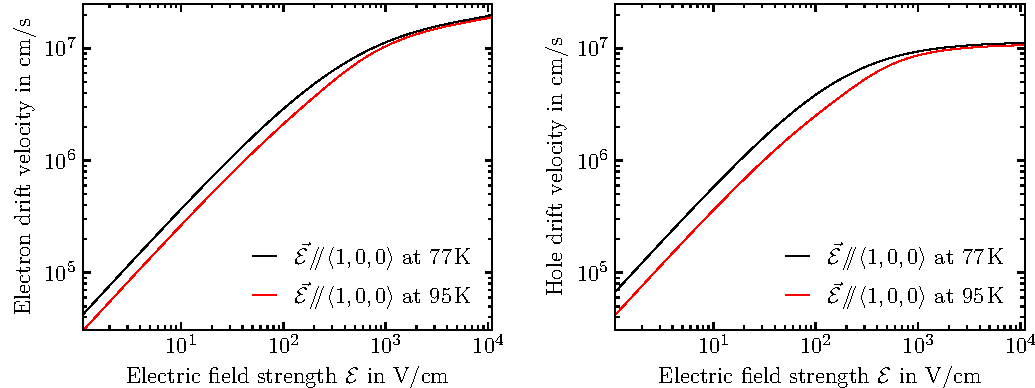
\includegraphics[width=6in]{figs/sim/drift_vel_temp_corr.pdf}
    \caption{Electron (left) and hole (right) drift velocity at 77\,K and 95\,K calculated using the procedure outlined in the text.}
    \label{fig:drift_vel_temp_corr}
\end{figure}

\section{Impurity Model}
Assuming a linear impurity gradient between the impurity concentrations provided by the detector vendor, $\rho_{\text{top}} = 1.109\times 10^{10}\,\text{cm}^{-3}$ and $\rho_{\text{bottom}} = 1.98\times 10^{10}\,\text{cm}^{-3}$, the simulated depletion voltage did not match the depletion voltage measured during biasing: 2950\,V. This model is referred to as the vendor impurity model in the text. Applying factor of 0.91 to $\rho_{\text{top}}$ and $\rho_{\text{bottom}}$ brings the simulation into agreement with this measurement. To simulate the thermal release of impurities from deep hole traps, a constant impurity concentration of $2.5\times10^9$\,cm$^{-3}$ was added to the scaled values. This value was chosen such that the simulated depletion voltage matches the ``settled'' depletion voltage, 3350\,V, which was measured going down from 3500\,V after multiple days of operation at this bias. The depletion impurity model is defined as the linear model between the scaled and offset values:
\begin{equation}
	\rho_\text{top,bottom}^\text{depletion} = 0.91\rho_\text{top,bottom}^\text{vendor} + 2.5\times10^9\,\text{cm}^{-3}~.
\end{equation}
Without additional information, this model represents ``a best estimate'' of the true impurity profile of the detector. As introduced in Chapter~\ref{chap:bubble}, the progress of the depletion surface can be used to provide a better estimate of the impurity profile. While depletion impurity model is based on one reference point -- the depletion voltage -- a new model was constructed to use the shape of the depletion surface at three additional reference points: 900\,V, 1200\,V and 3100\,V. This new model is referred to as the bubble impurity model. 
\begin{figure}[htb]
    \centering
    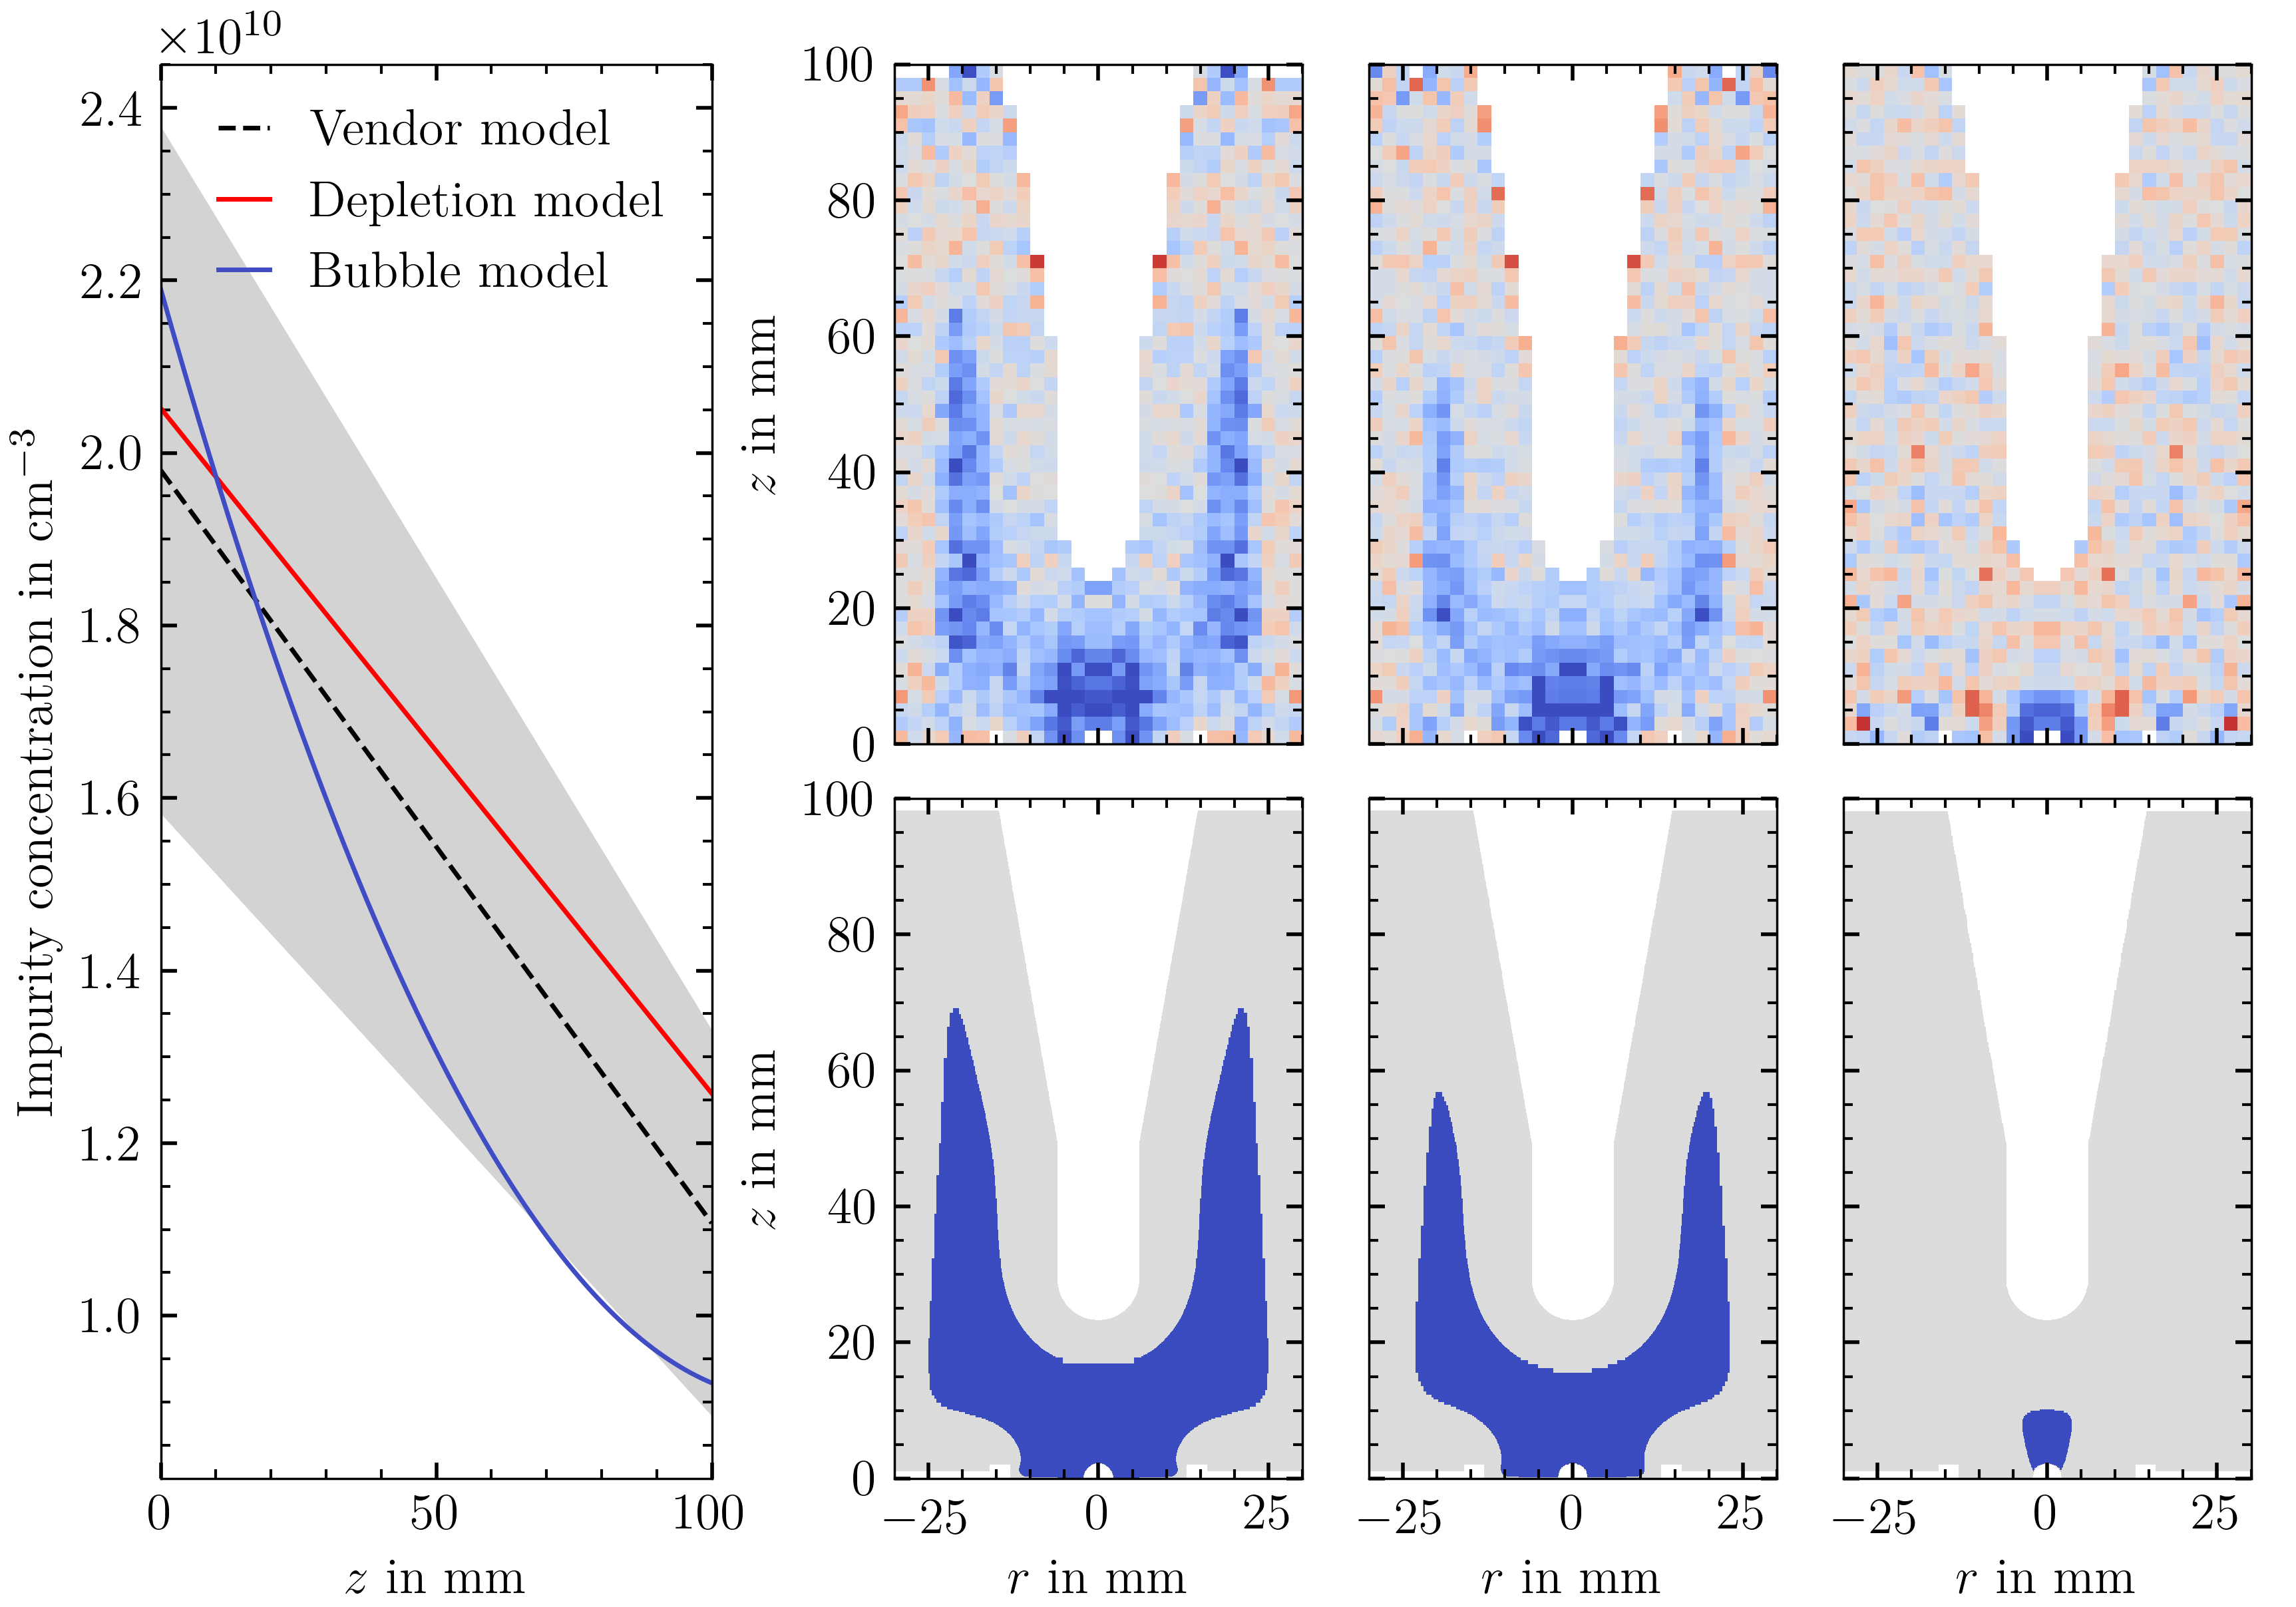
\includegraphics[width=6in]{figs/sim/bubbles_impurities.png}
    \caption{The vendor, depletion and bubble impurity models are shown on the left, with 20\% error band placed around the vendor model. This band represents the minimum uncertainty on the values reported by the vendor. Using the bubble model, the progress of the depletion surface in simulation (bottom right) was fit to data (top right).}
    \label{fig:bubbles_impurities}
\end{figure}

Although the progress of the depletion surface can be matched with a linear model, this pushes impurity concentrations at the ends of the detector far away from their vendor values. Thus, a quadratic model was adopted. \SSD{} was used to simulate the progress of the depletion surface with respect to the parameters of the quadratic model. The best fit was found with the following parameters:
\begin{equation}
	\rho^\text{bubble}(z) = 2.19\times10^{10}\,\text{cm}^{-3} - 2.27\times10^9\,\text{cm}^{-4}z + 1.00\times10^8\,\text{cm}^{-5}z^2~,
\end{equation}
where $z$ is measured from the point-contact end of the detector in cm. Note that the edges of the depletion surface in data are quite diffuse. Therefore, only the most salient features of the measured depletion surface, a single-valued outer $r$ and peak $z$, at given bias, were used for the fit. All three models, vendor, depletion and bubble are shown on the right of Fig.~\ref{fig:bubbles_impurities}. 

\section{ICPC Detector Response} \label{sec:ic_sims}
The detector response was simulated with the bubble impurity model at 3500\,V bias. The simulated electric field and weighting potential are shown in Fig.~\ref{fig:icpc_fields}.
\begin{figure}[htb]
    \centering
    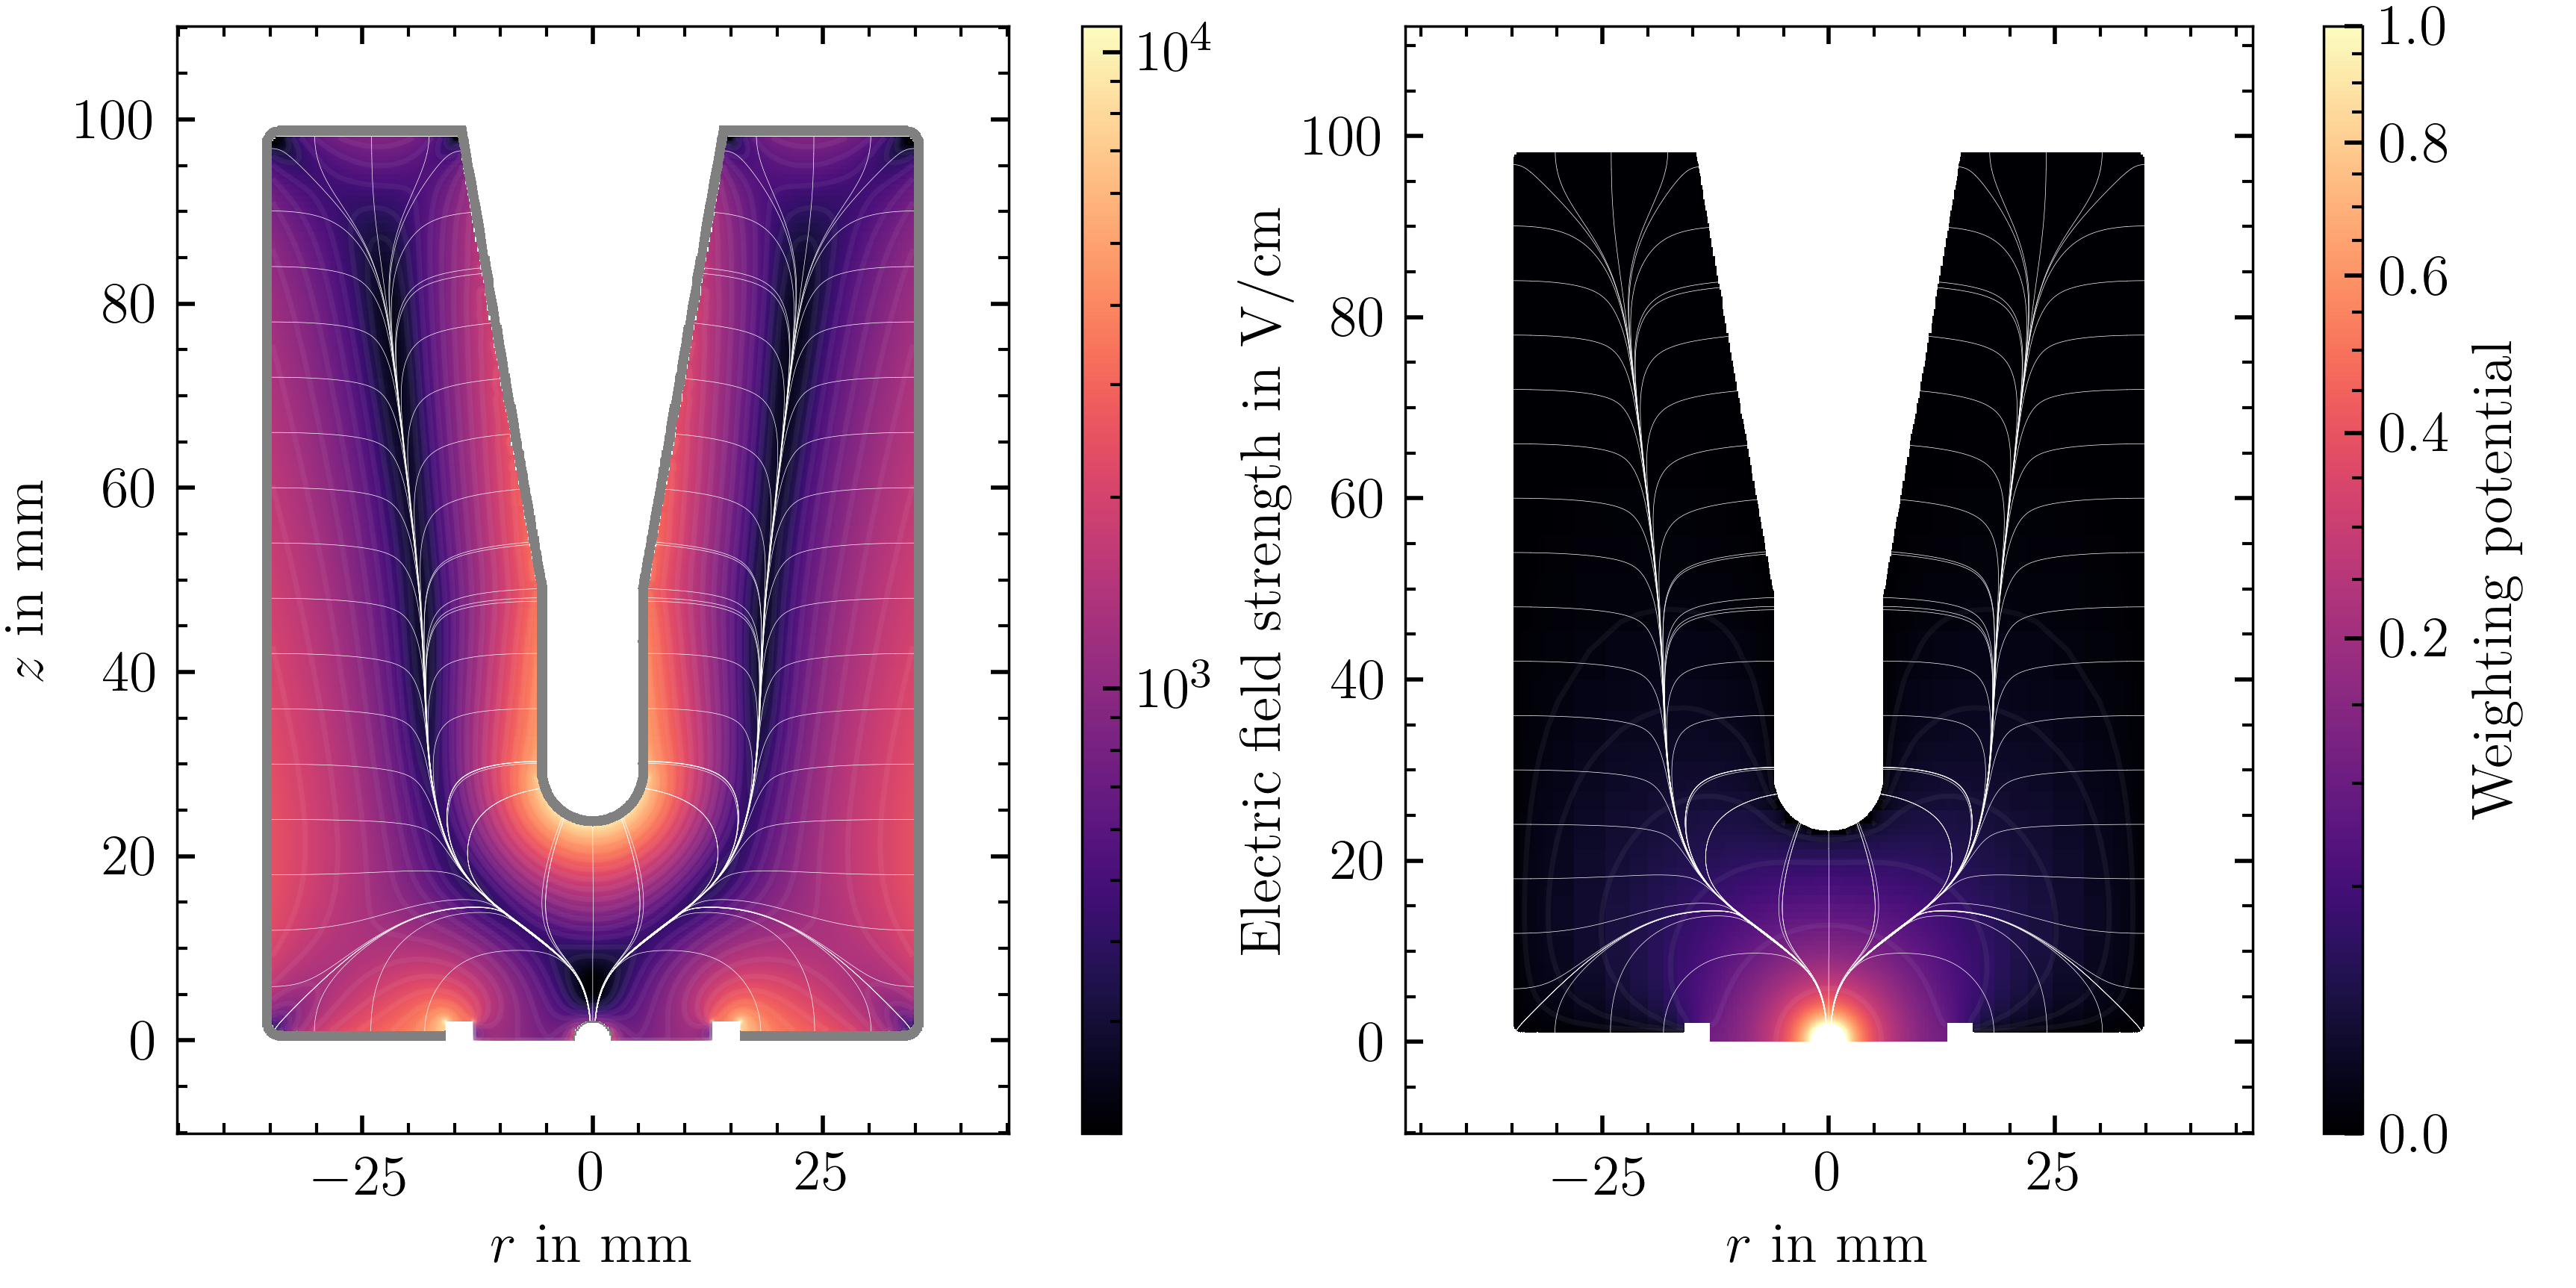
\includegraphics[width=6in]{figs/sim/icpc_fields_3500V.png}
    \caption{The electric field magnitude and weighting potential of the ICPC at 3500\,V bias are shown on the left and right respectively. Thin vertical electric field lines are drawn in white. Six contour lines are plotted for the weighting potential, corresponding to values given by $10^n$ where $n$ varies between -3.5 to -0.5 in steps of 0.5.}
    \label{fig:icpc_fields}
\end{figure}

Hole drift velocity saturates above 200\,V/cm for the temperature of interest. At 3500\,V, the simulated electric field magnitude is above this value for almost the entire detector, except for a small strip at $r = 18$\,mm between $z = 30$ and 52\,mm. Such areas were targeted to in the search for regions of high charge trapping. However, as was shown in Chapter~\ref{chap:trapping}, there is no evidence of significant charge trapping throughout the bulk.  

Charge drift was simulated with the calculated electric field and the drift velocities established at 95\,K. Hole drift times dominate for the majority of the detector, except for a small region close to the p$^+$ contact. This is seen in the drift time map of the $\left<1\,1\,0\right>$ axis in Fig.~\ref{fig:icpc_drifttimes}. The maximum drift time at 3500\,V bias is 2.2\,$\upmu$s. This value set a lower bound for the flat time of the trapezoidal filter used for energy estimation in Sec.~\ref{sec:energy}.
\begin{figure}[htb]
    \centering
    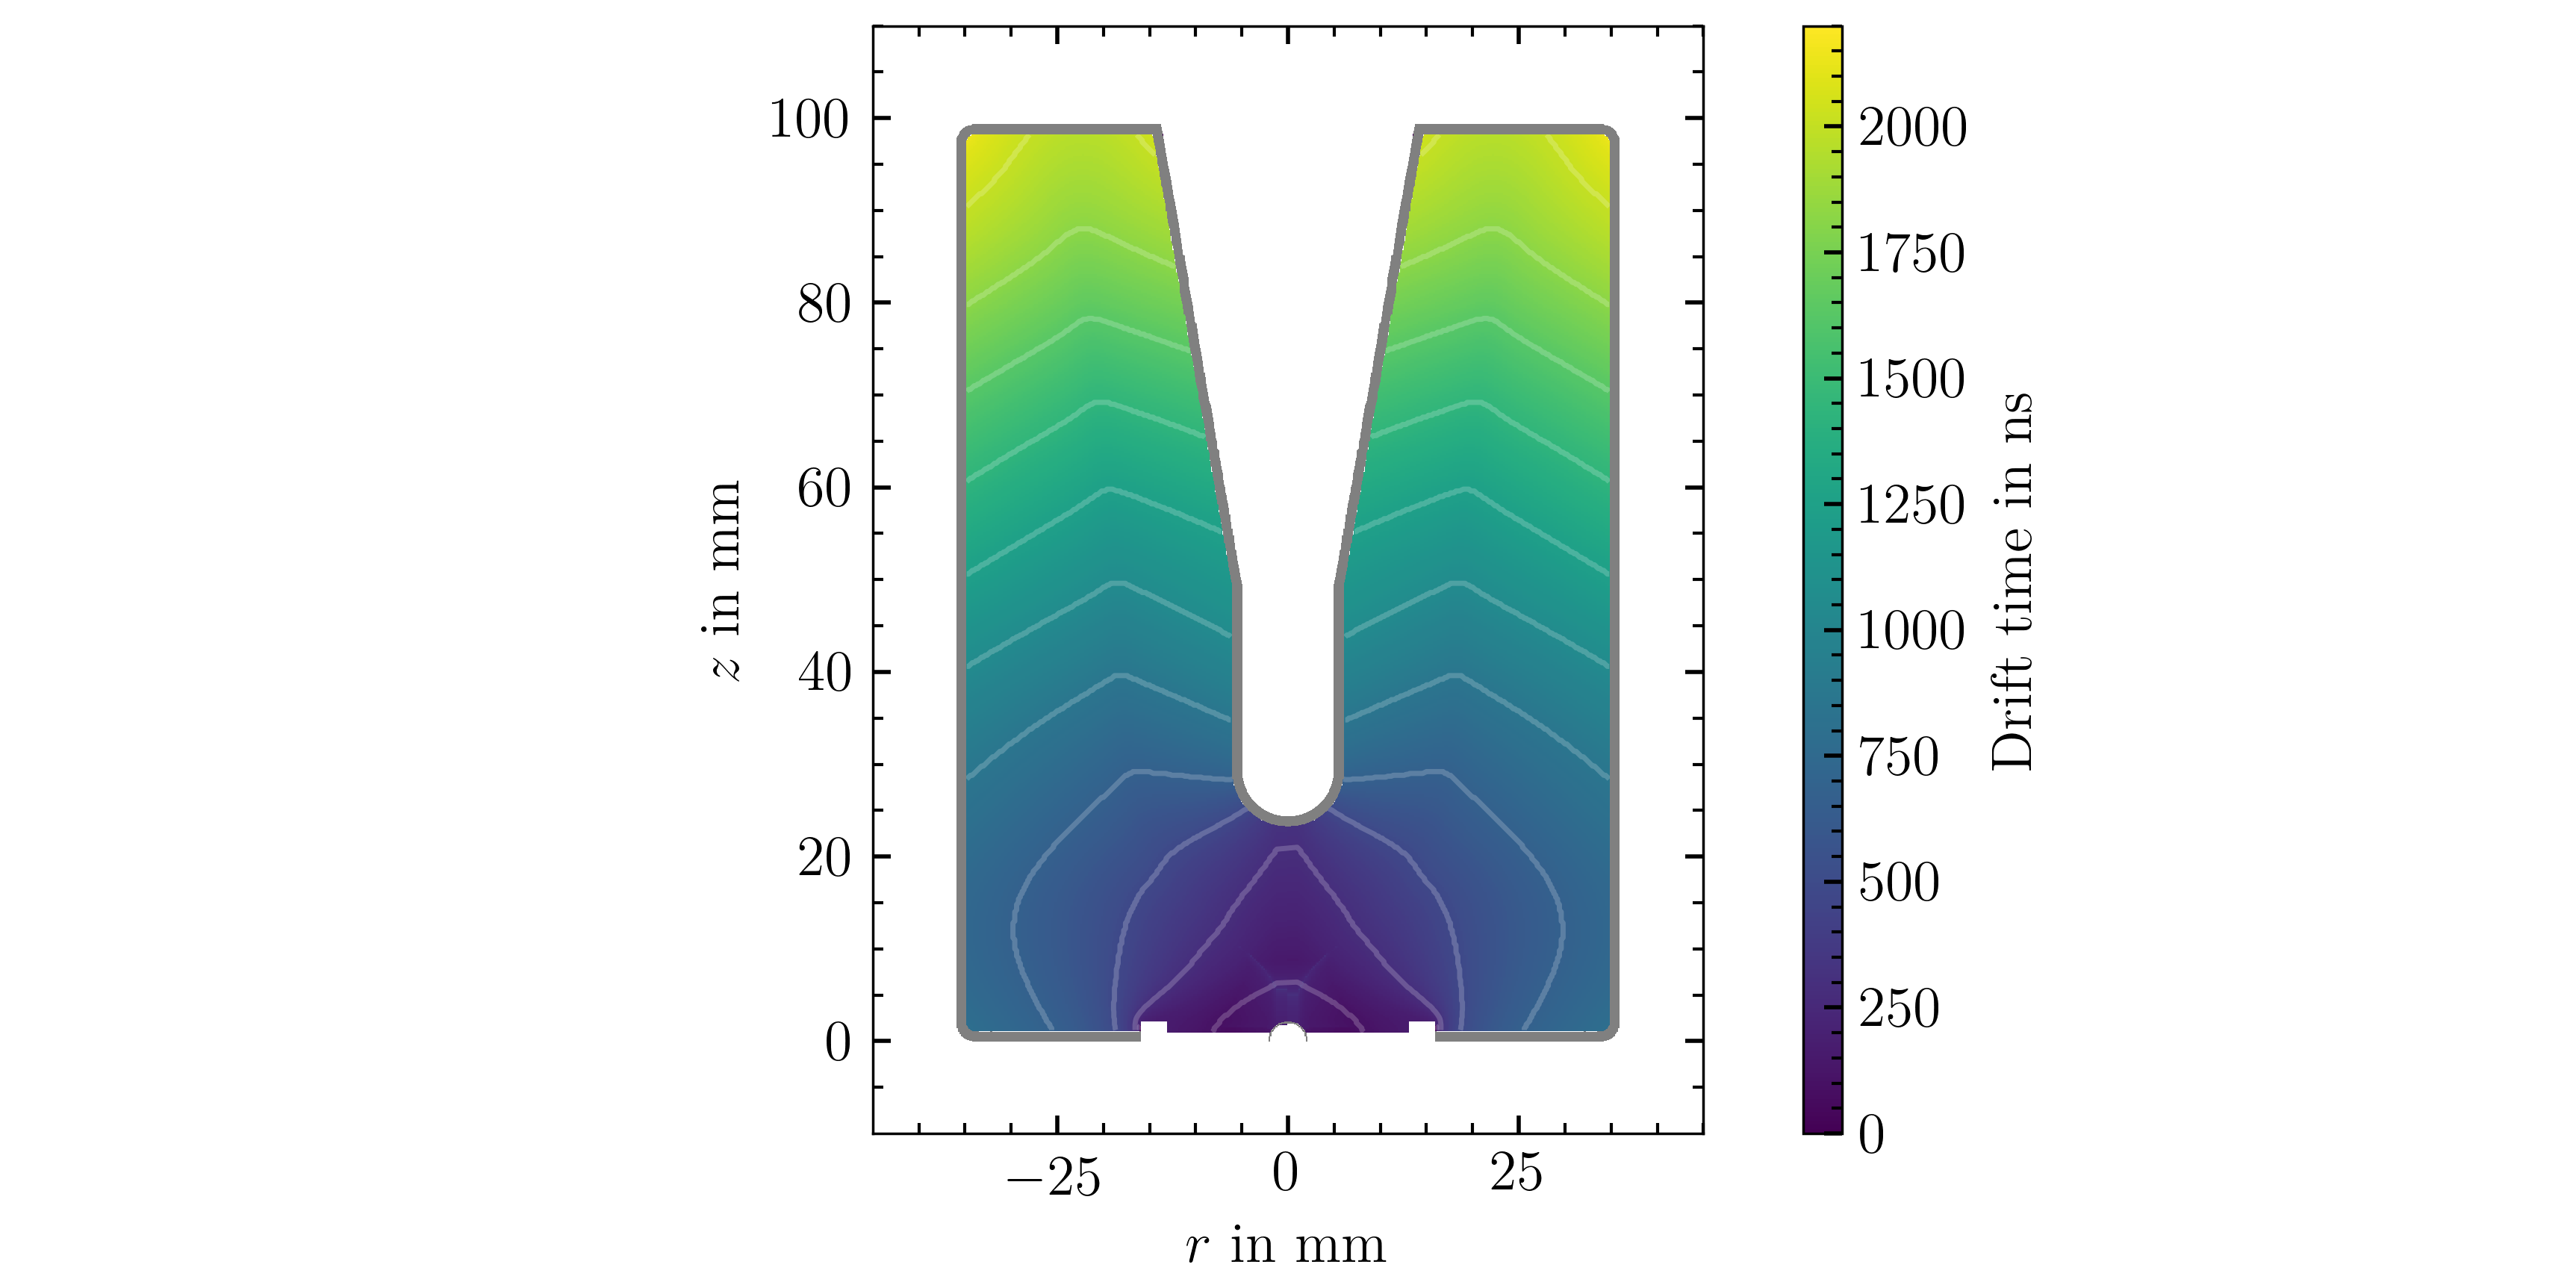
\includegraphics[width=6in]{figs/sim/icpc_drifttimes.png}
    \caption{The drift time along the $\left<1\,1\,0\right>$ axis of the ICPC at 3500\,V bias is shown. Isochrones for \textit{hole} drift times are drawn every 200\,ns starting at the line closest to the p$^+$ contact at 100\,ns.}
    \label{fig:icpc_drifttimes}
\end{figure}

\clearpage 

\section{Voxelation}
In data, raw detector pulses are amplified and shaped by the electronics. Recorded pulses that fall within a voxel are combined into a superpulse, effectively averaging the spread of point-like pulse shapes expected in this volume. Both of these effects, electronics response and voxelation, are applied in simulation. 

To simulate the spread in pulse shapes within a voxel, the charge cloud generation algorithm of \SSD{} was used. This algorithm spawns evenly distributed point-like charges in a sphere of a given radius. The diameter of the sphere was set equal the side of a voxel, and 200 charges were spawned per voxel as the left panel of Fig.~\ref{fig:voxelation} shows.
\begin{figure}[htb]
    \centering
    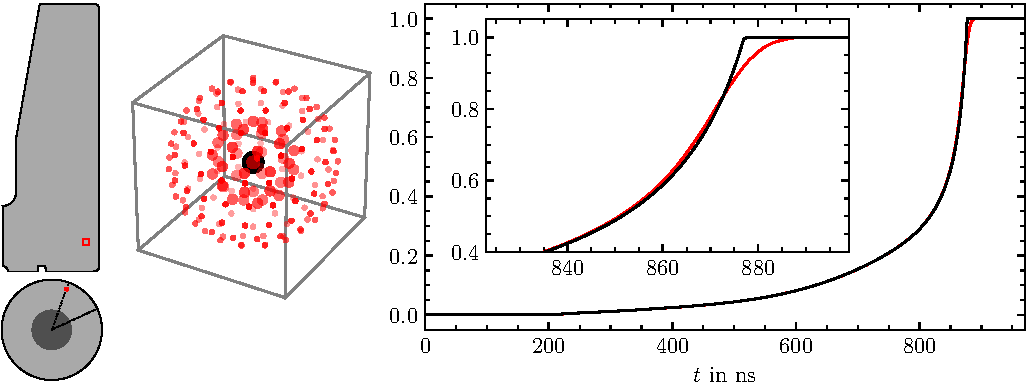
\includegraphics[width=6in]{figs/sim/voxelation.pdf}
    \caption{The pictogram shows the location of a $(2\times2\times2)$\,mm voxel in the detector. The superpulse resulting from energy depositions at the red points in the voxel is shown in red on the left, whereas the pulse resulting from an energy deposition at the centroid is shown in black. The size of the red points represents the share of total charge assigned by the charge cloud generation algorithm.}
    \label{fig:voxelation}
\end{figure}

The signals for every charge were calculated and combined by the charge cloud algorithm, leading to a simulated superpulse. Points closer to the center of the voxel carry more charge, and thus have a greater weight when combined to form the superpulse. In reality the distribution of energy depositions in the voxel is expected to be approximately Gaussian in all spatial dimensions (accounting for the expected beam profile and reconstructed $z_\theta$ error). In this respect, the concentration of charge at the center of the voxel given by charge cloud algorithm approximates this expected distribution well. Nevertheless, to better approximate the real energy deposition distribution, a selected number of voxels were simulated with 10000 random point-like charges with the expected Gaussian distribution in all spatial dimensions. Since no significant pulse shape discrepancies were found with respect to using the charge cloud generation algorithm, the latter was adopted to save computation time. However, there is a significant deviation -- as the right panel of Fig.~\ref{fig:voxelation} exemplifies -- between a voxel's superpulse and a pulse generated by a drifting a point-like charge from its centroid. 

\section{Electronics Response}\label{sec:electronicsanalytical}

To simulate the effect of the readout electronics, the simulated superpulses were convolved with the electronics response function determined in Sec.~\ref{sec:electronicsresponse}. Since convolution is distributive, this can be done at the superpulse level, instead of acting on individual pulses from point-like charges. The application of the electronics response function accounts for the limited bandwidth of the preamplifier, an effect which is most succinctly observed in fast rising near-p$^+$ events. In such events, convolution with the electronics response function results in considerably longer measured drift times. The observed overshoot from waveform maximum is also introduced by the electronics. 

Once convolved with the measured electronics response function, simulated and measured pulse shapes were compared for each voxel. The pulse shapes did not agree. In particular, the maximum current amplitudes, $A$, of measured pulses, were a factor of five lower than in simulation. Prior to electronics model application, differences in $A$ may arise from two main sources of uncertainty in the simulation:
\begin{itemize}
	\item Drift velocities (at a given electric field strength and temperature) vary up to 30\% in literature~\cite{driftvelGe,drift_pars,drift_parametrization,siggen}. The simulation is thus affected by the choice of drift parameterization and corresponding parameters.
	\item The impurity concentrations at the ends of the detector quoted by the manufacturer carry an $>20$\% uncertainty. 
\end{itemize}
As expected, a systematic variation of drift velocities and impurity concentrations within uncertainties did not come close to accounting for the difference in $A$. Thus, the difference must originate in the electronics. In conclusion, the measured electronics response function does not model the effect of the electronics on real signals (as opposed to signals from the pulser input of the preamplifier) properly. 
\begin{figure}[htb]
    \centering
    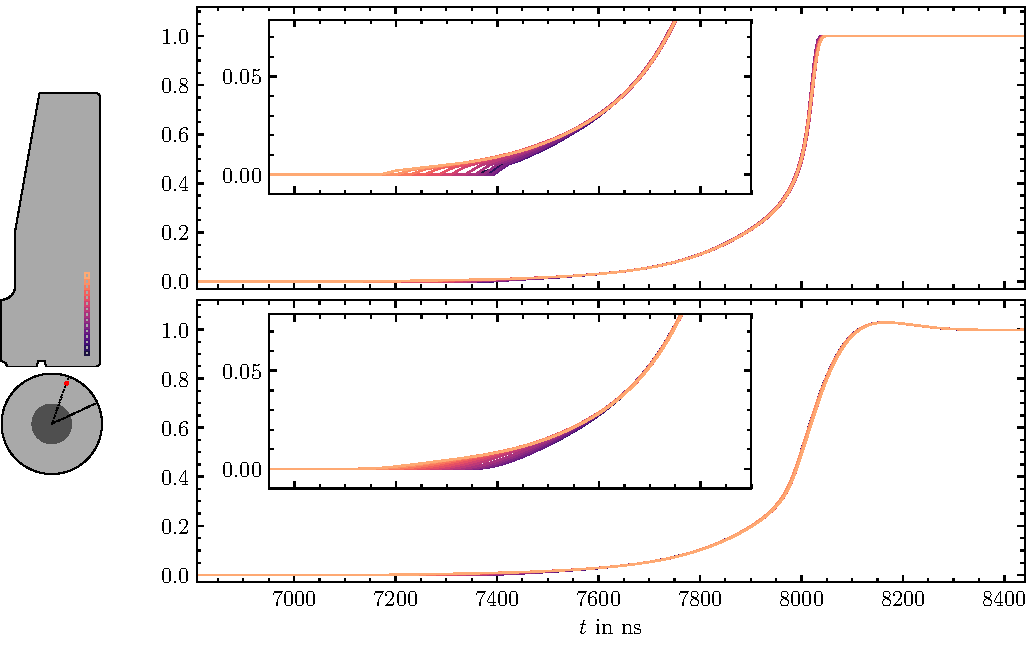
\includegraphics[width=6in]{figs/sim/electronics_response_application.pdf}
    \caption{The simulated $(r = 31, z = [5,33])$\,mm, $\left<1\,1\,0\right>$, HV = 3500\,V superpulses are depicted, with an inset (with matching $x$-scale) showing a close up of the start of the rise. Eq.~\ref{eq:second_order_low_pass} is convolved with the superpulses at the top to produce the superpulses at the bottom.}
    \label{fig:electronics_response_application}
\end{figure}

Two analytical electronics response models were considered in place of the measured one. The effect of the preamplifier bandwidth was first modeled as a single RC-integration time constant, $\tau$. Using $\tau = 70$\,ns led to the desired $A$. However, the rise times resulting from the use of this model were considerably longer than those seen in data, in particular close to the point contact. Therefore, a second model was considered. A RC-integrator is a first order low-pass filter. This model was taken to the next order, assuming the form of a second order Butterworth filter~\cite{Butterworth1930}. The transfer functions (using Laplace variable $s$) of the first and second order low-pass filters are shown in Eq.~\ref{eq:first_order_low_pass} and Eq.~\ref{eq:second_order_low_pass} respectively, where the inverse Laplace transform has been taken to yield the corresponding electronics response functions. Note that the cuttoff frequency of these filters is given by $1/2\pi\tau$. 
\begin{equation}
		\mathscr{L}^{-1}\left(\frac{1}{s\tau + 1}\right) = \frac{1}{\tau}e^{-t/\tau}
	\label{eq:first_order_low_pass}
\end{equation}
\begin{equation}
	\mathscr{L}^{-1}\left(\frac{1}{s^2\tau^2 +\sqrt{2}s\tau + 1}\right) = \frac{\sqrt{2}}{\tau}\sin\left(\frac{t}{\sqrt{2}\tau}\right)e^{-t/\sqrt{2}\tau}
	\label{eq:second_order_low_pass}
\end{equation}
The best match between simulated and measured $A$ was obtained with the second order filter with $\tau = 47$\,ns. Superpulses before and after application of this model are shown in the top and bottom panels of Fig.~\ref{fig:electronics_response_application} respectively.

The imaginary poles of transfer function of the second order filter introduce the desired overshoot from waveform maximum and the following oscillations seen in data, giving a closer approximation in overall pulse shape. Moreover, the rise time from simulation and data also match reasonably well over most of the area covered by the radial scans. Therefore, this model was adopted and used in the simulation chain. A side-by-side comparison of $A$ and rise time is shown in Fig.~\ref{fig:AOE_fast_axis_data_sim_comp} and Fig.~\ref{fig:DT_fast_axis_data_sim_comp} respectively. 
\begin{figure}[H]
    \centering
    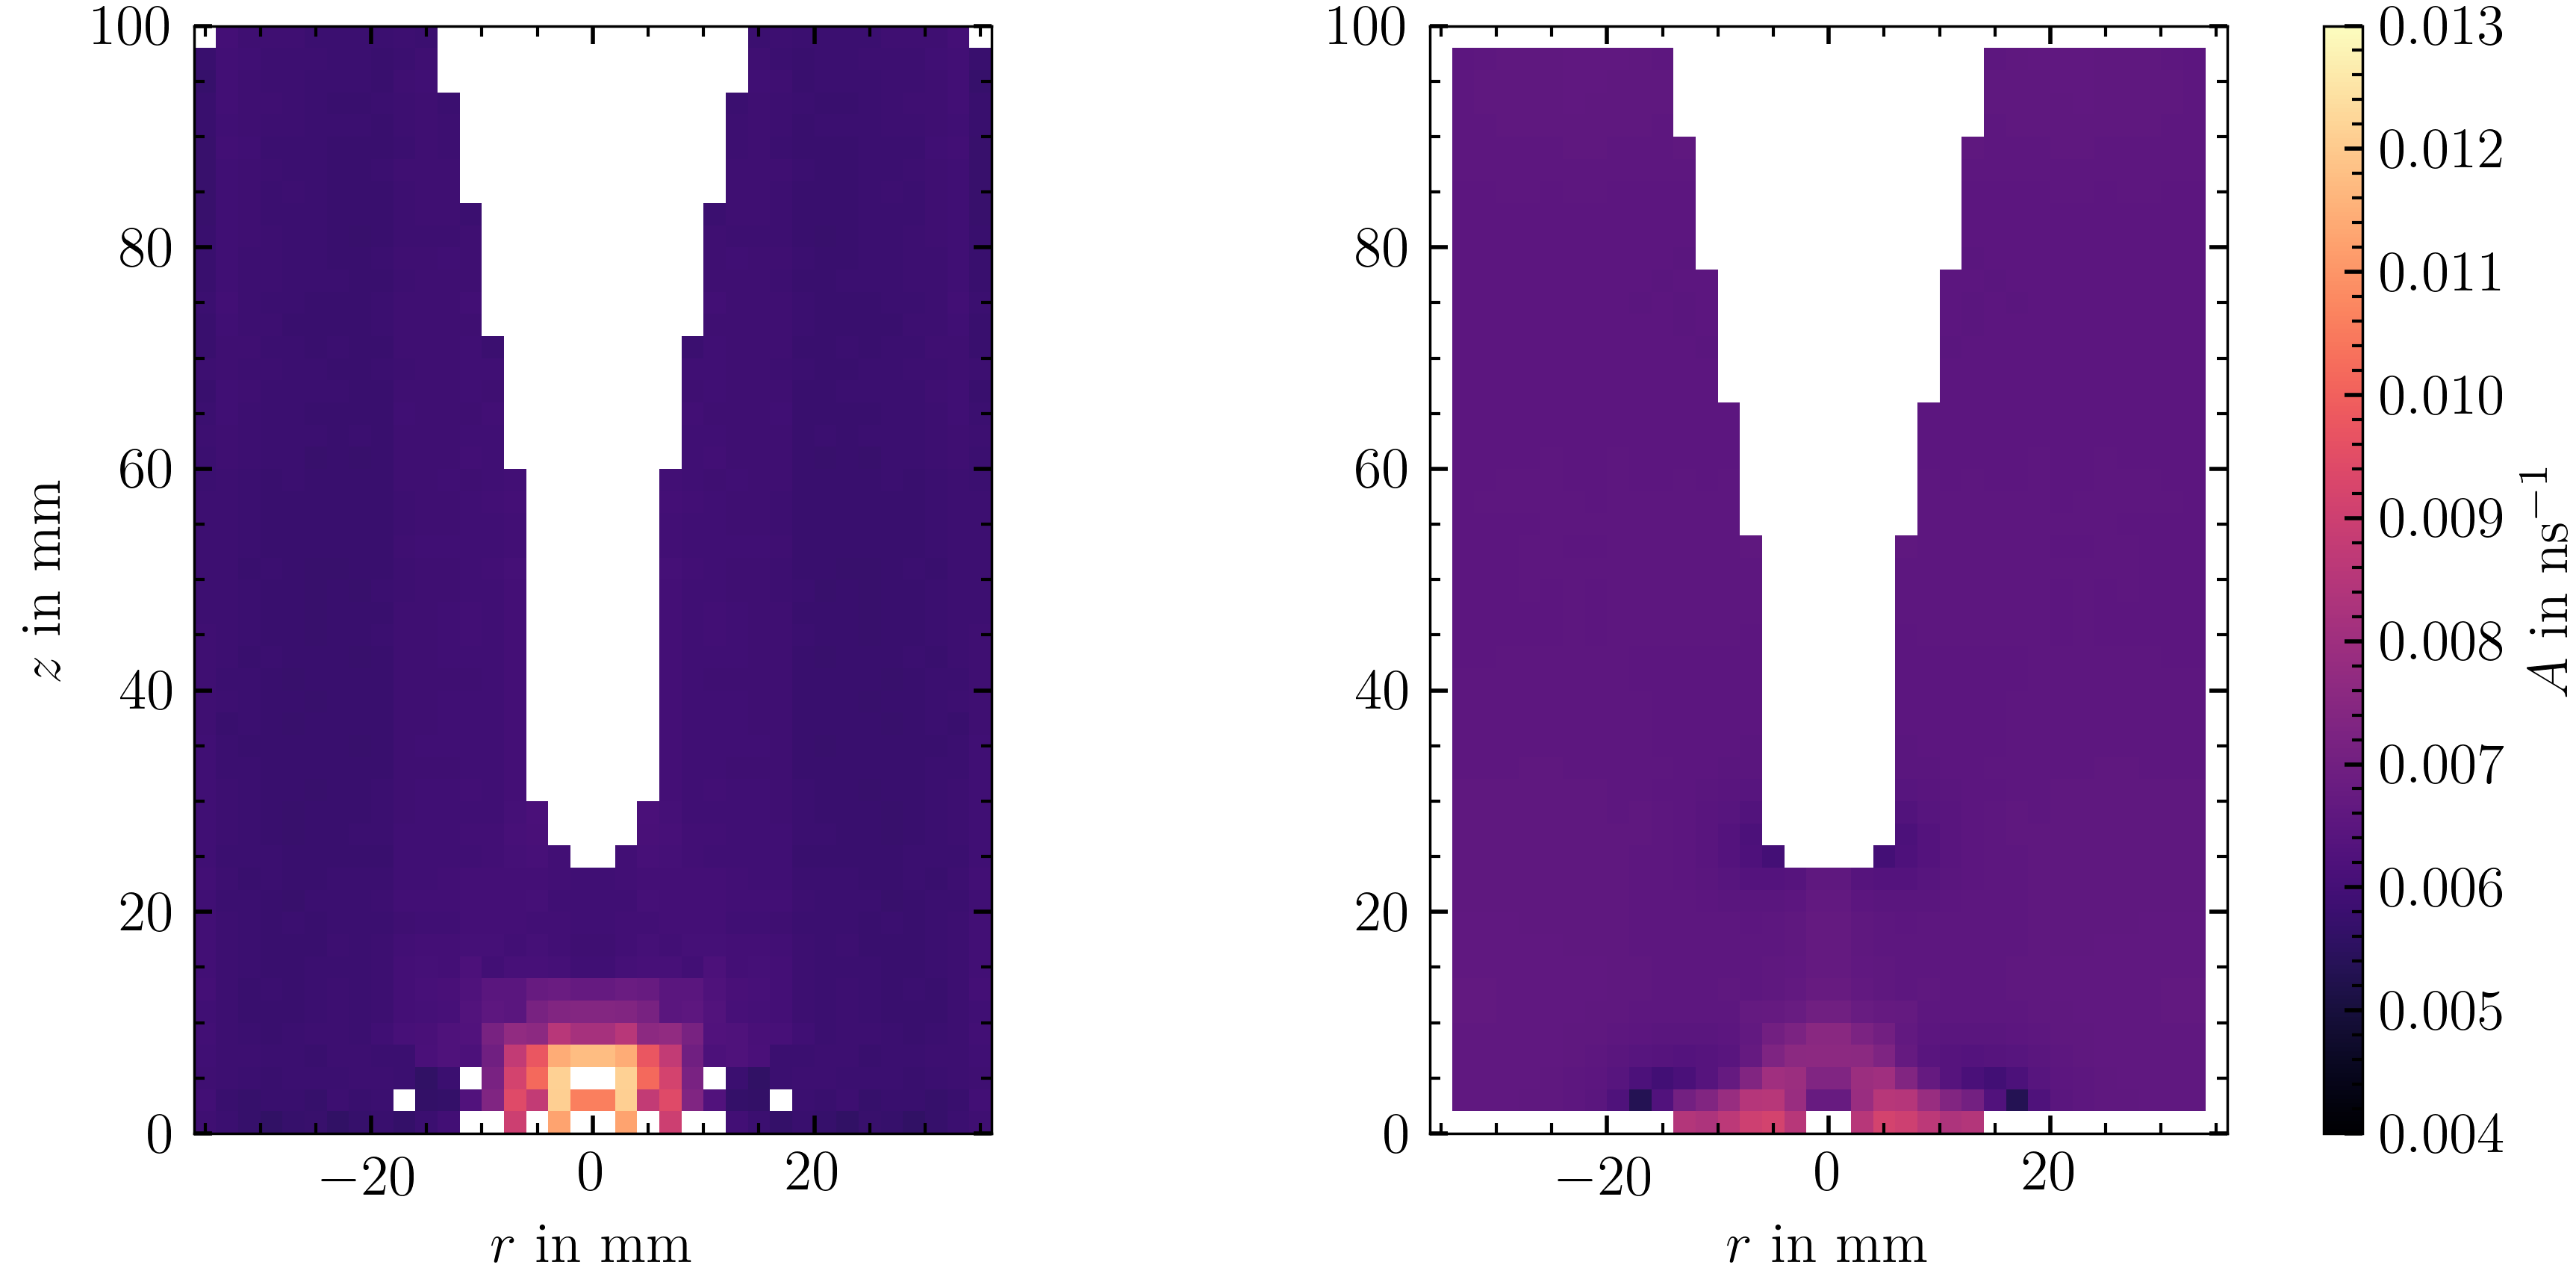
\includegraphics[width=6in]{figs/sim/AOE_fast_axis_data_sim_comp.png}
    \caption{The current amplitudes from data and simulated superpulses are shown on the left and right respectively for the $\left<1\,0\,0\right>$-axis of the detector at 3500\,V. The simulation uses the bubble impurity model and electronics modeled as the second order Butterworth filter with $\tau = 47$\,ns. The data heatmaps has been mirrored to include the (unscanned) radial slice at $\phi+180^\circ$.}
    \label{fig:AOE_fast_axis_data_sim_comp}
\end{figure}

As in simulation, $A$ in data is constant everywhere in the bulk except very close to the point-contact. The measured $A$ in this constant region is approximately 15\% lower than in simulation. On the other hand, as seen from the 0.3-99.7\% rise times, simulated pulses are approximately 10\% faster than in data. The same level of discrepancy was observed in a Compton scan of the fast axis of a p-type segmented detector at 78\,K~\cite{felix_masters}. Nevertheless, rise times agree in trend. In particular, the 0.3-99.7\% rise time becomes constant for the top two-thirds of the detector in data and simulation. 
\begin{figure}[H]
    \centering
    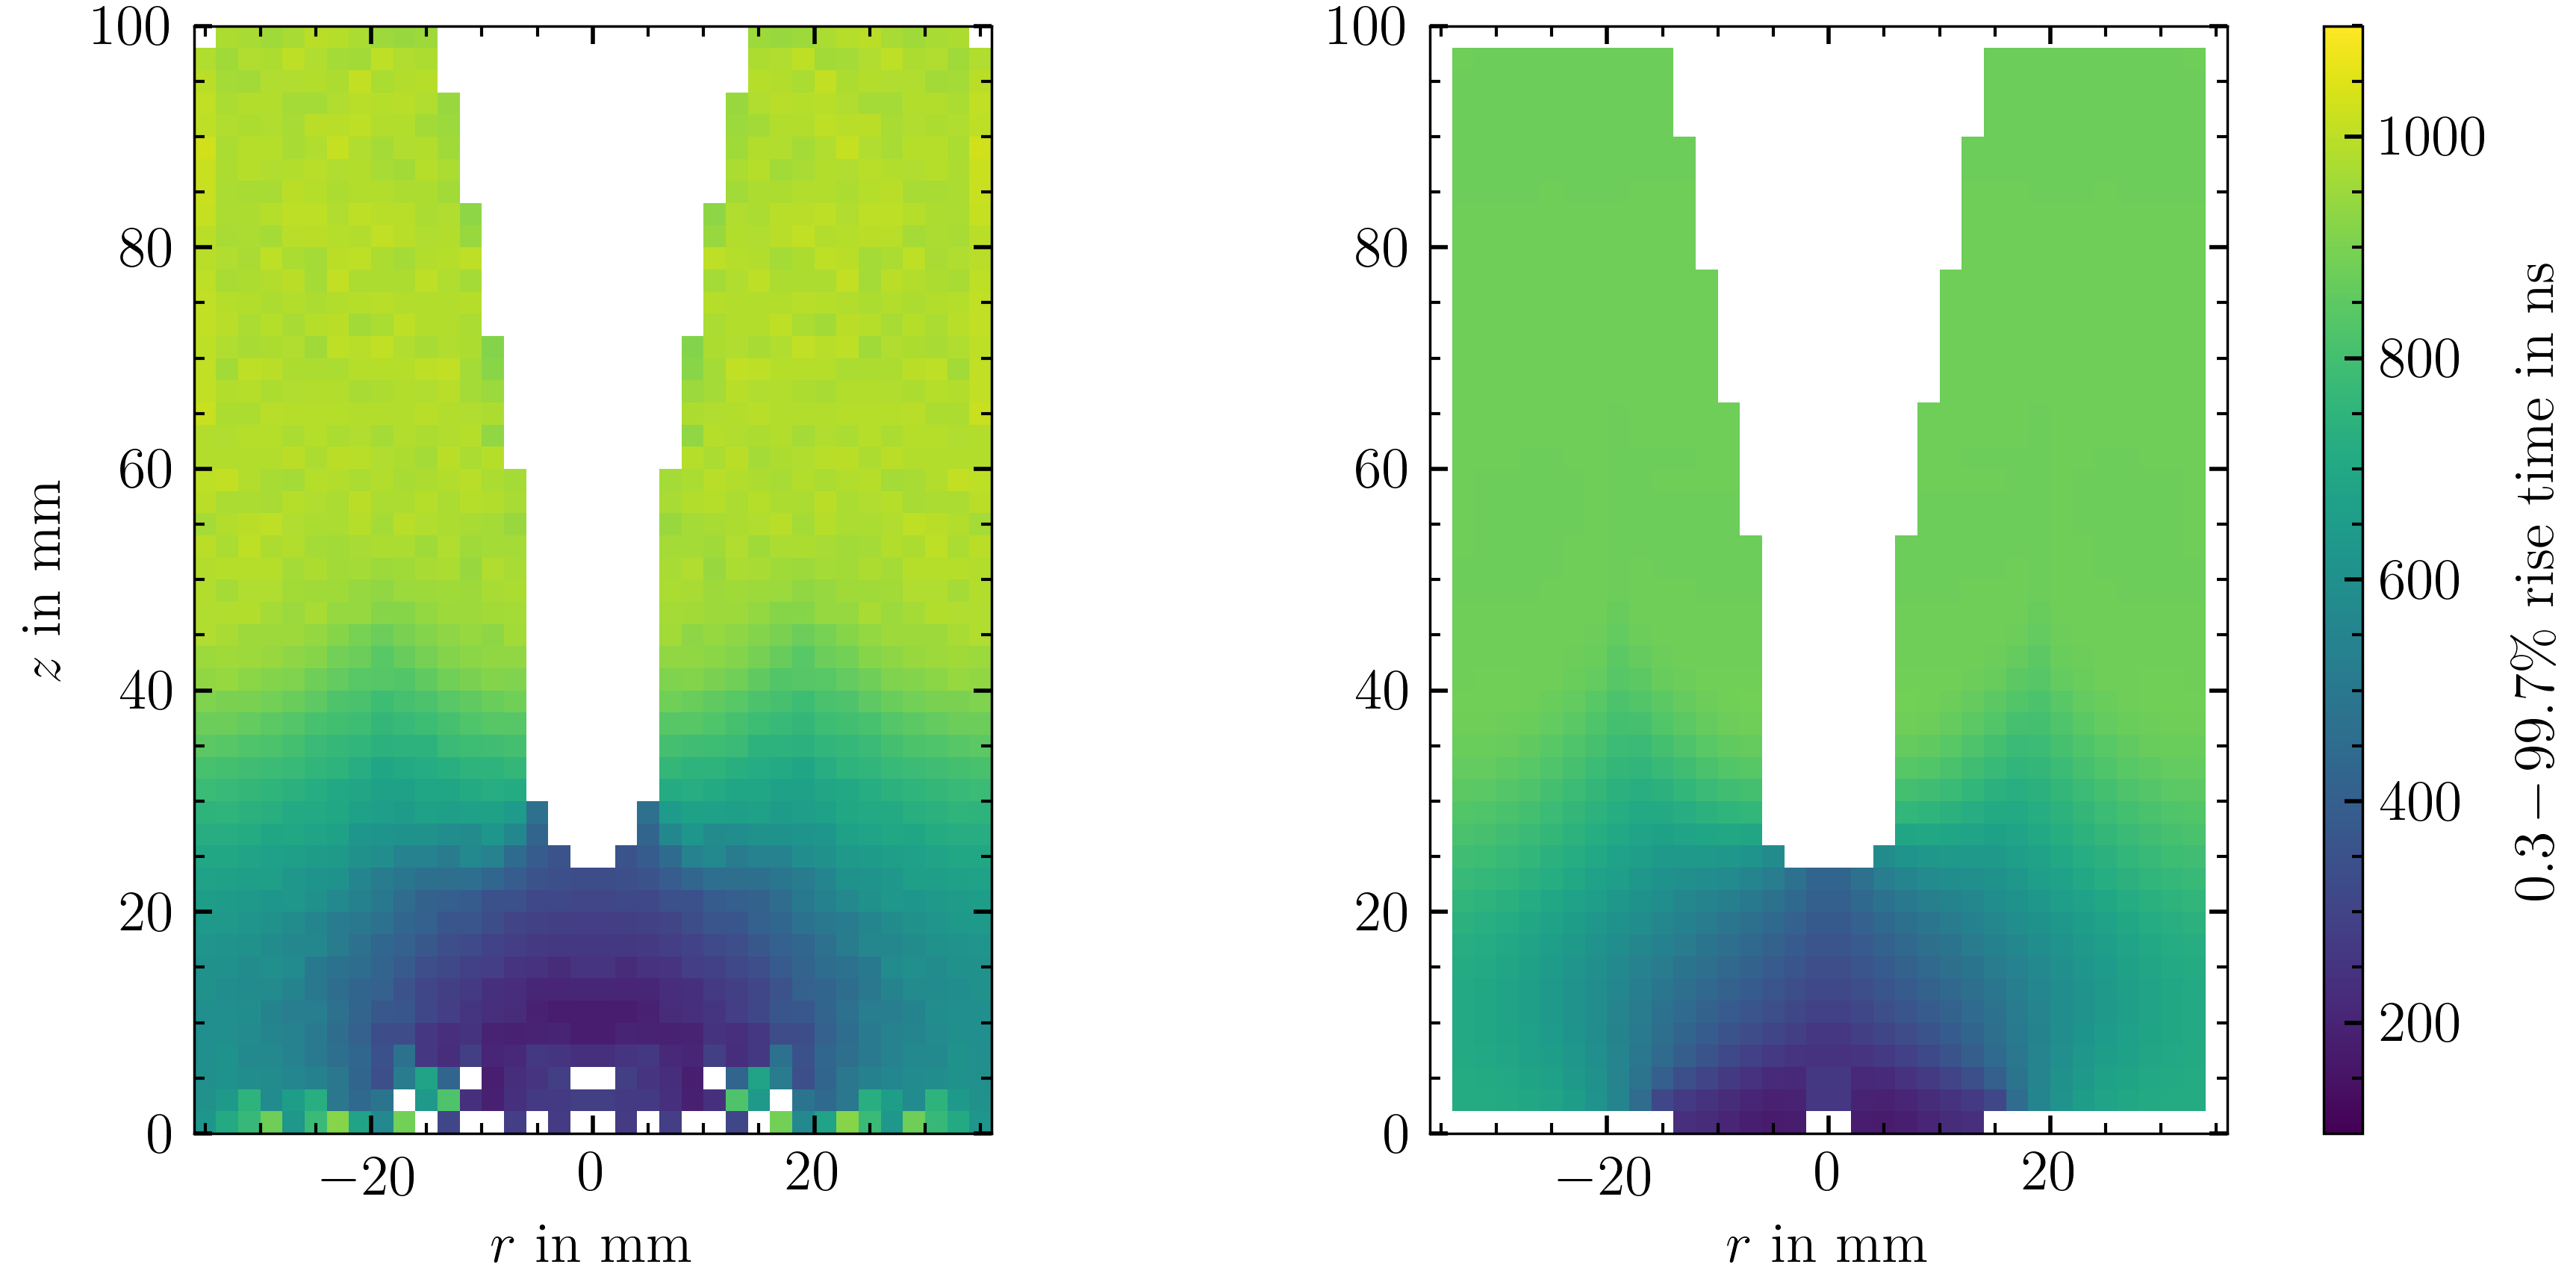
\includegraphics[width=6in]{figs/sim/DT_fast_axis_data_sim_comp.png}
    \caption{The 0.3-99.7\% rise times from data and simulated superpulses are shown on the left and right respectively for the $\left<1\,0\,0\right>$-axis  of the detector at 3500\,V. The simulation uses the bubble impurity model and electronics modeled as the second order Butterworth filter with $\tau = 47$\,ns. The data heatmap has been mirrored to include the (unscanned) radial slice at $\phi+180^\circ$.}
    \label{fig:DT_fast_axis_data_sim_comp}
\end{figure}

\section{Pulse Shape Comparison of Depletion and Bubble Models}\label{sec:impcomp}

Using the analytical electronics response function determined in Sec.~\ref{sec:electronicsanalytical}, a direct comparison between pulse shape from data and simulation was made. The measured pulse shape is most trusted for the top half of the detector arms. In this region, over 50 2-hit pulses were collected per voxel. Additionally, above 80\% of these 2-hit pulses survived the self-similarity cut, indicating a low level of misreconstructed events prior to their removal. The pulses in the top half of the arms are very similar to each other, thus the conclusions drawn from one voxel may be applied to all voxels in this region. Thus, one of these, specifically the ($r = 31$, $z = 81$)\,mm, voxel, was chosen to evaluate the depletion and bubble impurity models. The simulated superpulses based on these models are shown in relation to the measured superpulse in Fig.~\ref{fig:model_comparison}. 
\begin{figure}[htb]
    \centering
    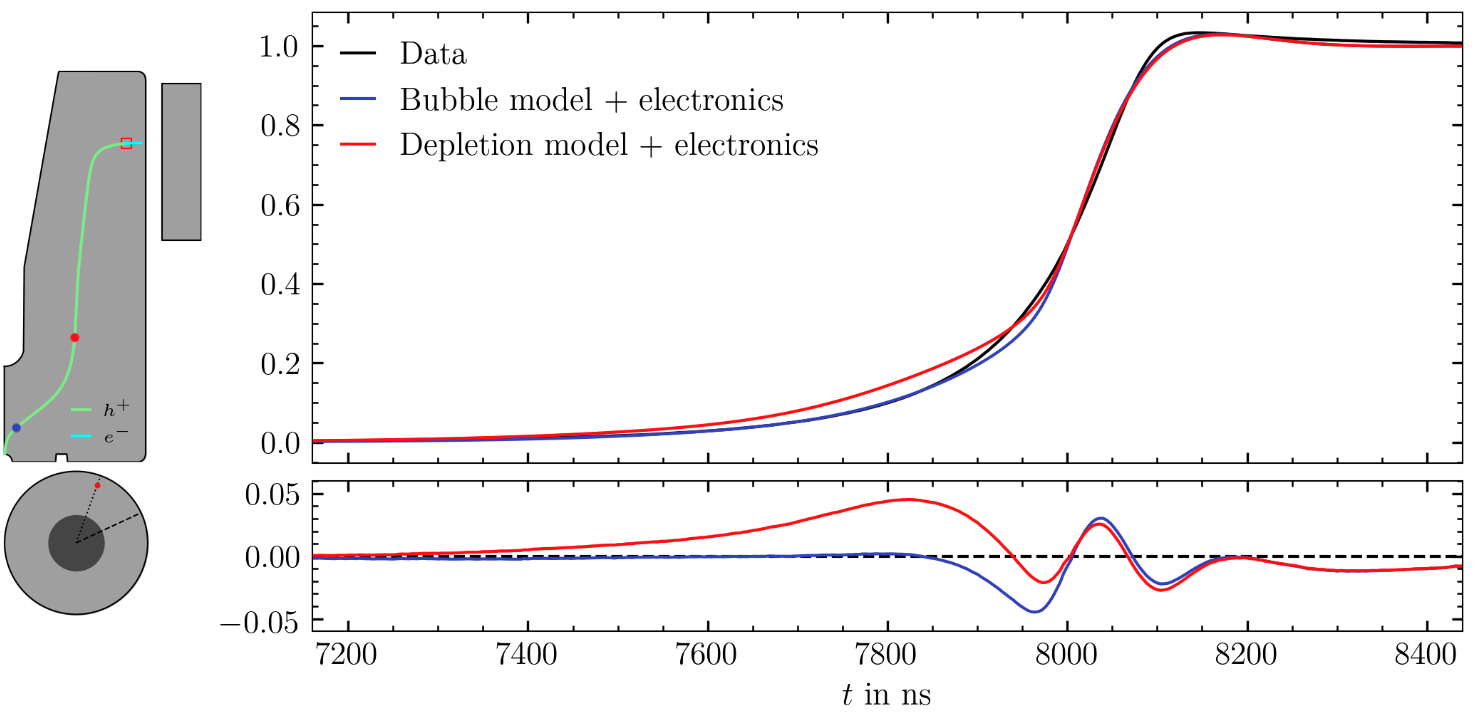
\includegraphics[width=6in]{figs/sim/model_comparison.png}
    \caption{The measured superpulse from the ($r = 31$, $z = 81$)\,mm voxel is shown in relation to two simulated superpulses, with the residuals shown at the bottom. The first (red) is based on the depletion impurity model, while the second (blue) is based on the bubble impurity model. The second order Butterworth filter with $\tau = 47$\,ns modeled the electronics in both cases. The simulated drift paths of electrons and holes is shown on the pictogram. A red dot and blue dot on the drift path mark the location where data and simulation diverge. These locations are estimated as described in the text.}
    \label{fig:model_comparison}
\end{figure}

As seen from the residuals, the bubble impurity model results in a better overall agreement between data and simulation. A very close agreement in pulse shape is obtained up to approximately 200\,ns before full charge collection. For the depletion model, this agreement is only found until approximately 800\,ns before full charge collection. The location of holes at these times were simulated (by stepping back from the end of the drift) and are plotted using the same color code on the pictogram of Fig.~\ref{fig:model_comparison}. In conclusion, the bubble model provides a better estimate of the impurity profile of the detector, and is thus adopted for the simulated pulse shape library. These superpulses are shown alongside their measured counterparts in the next chapter. 

However, the pulses simulated employing the bubble model are not in complete agreement with data. This can occur for a myriad of reasons, and each should be studied in turn. The list that follows explores the limitations of the simulations and the major sources of uncertainty. 
\begin{itemize}
	\item Only a few features of the depletion surface were used to fit the impurity model. With additional reference voltages and increased statistics at each one, the entire shape of the depletion surface can be used. This would allow for the introduction of radial gradients in the impurity model and in particular a precise modeling of the impurity profile close to the point contact. It is close to this point where simulated and measured pulse-shapes differ the most. 
	\item There is a 1.6$^\circ$ uncertainty in crystal axis orientation. As the next chapter expands upon, the true orientation may fall out of these bounds. Thus, off-axis effects must be considered. In particular transverse drift anisotropy could slow down pulses as they near the point contact. However, simulations show that for pulses originating in the top two-thirds of the detector this effect is small, with radial drift forming an up to 10$^\circ$ angle with the electric field. 
	\item The form of the electronics response model is assumed and fit to data rather than measured. 
	\item There is no established drift velocity temperature model.
	\item Charge drift velocities differ significantly in literature. However, by constraining all other uncertainties, corrections to drift velocities may be found by comparing simulated and measured pulse shapes.
\end{itemize}  